\documentclass[preprint,12pt]{elsarticle}
\usepackage{geometry}
%\geometry{letterpaper}                   % ... or a4paper or a5paper or ...
\usepackage{graphicx}
\usepackage{xspace}
\usepackage{amssymb} 
\usepackage{epstopdf}
 
  
\usepackage{datatool}
\usepackage{tikz}
\usepackage{pgfplots}
\usepackage{pgfplotstable}
\usetikzlibrary{patterns}
\usepackage{lscape} 
\usepackage{subfig}
\usepackage{multirow} 
\usepackage{rotating}


%% Use the option review to obtain double line spacing
%% \documentclass[preprint,review,12pt]{elsarticle}
   
%% Use the options 1p,twocolumn; 3p; 3p,twocolumn; 5p; or 5p,twocolumn
%% for a journal layout: 
%% \documentclass[final,1p,times]{elsarticle}
%% \documentclass[final,1p,times,twocolumn]{elsarticle}
%% \documentclass[final,3p,times]{elsarticle}
%% \documentclass[final,3p,times,twocolumn]{elsarticle}
%% \documentclass[final,5p,times]{elsarticle}
%% \documentclass[final,5p,times,twocolumn]{elsarticle}

%% if you use PostScript figures in your article
%% use the graphics package for simple commands
%% \usepackage{graphics}
%% or use the graphicx package for more complicated commands
%% \usepackage{graphicx}
%% or use the epsfig package if you prefer to use the old commands
%% \usepackage{epsfig}

%% The amssymb package provides various useful mathematical symbols
\usepackage{amssymb}
%% The amsthm package provides extended theorem environments
%% \usepackage{amsthm}

%% The lineno packages adds line numbers. Start line numbering with
%% \begin{linenumbers}, end it with \end{linenumbers}. Or switch it on
%% for the whole article with \linenumbers after \end{frontmatter}.
%% \usepackage{lineno}

%% natbib.sty is loaded by default. However, natbib options can be
%% provided with \biboptions{...} command. Following options are
%% valid:

%%   round  -  round parentheses are used (default)
%%   square -  square brackets are used   [option]
%%   curly  -  curly braces are used      {option}
%%   angle  -  angle brackets are used    <option>
%%   semicolon  -  multiple citations separated by semi-colon
%%   colon  - same as semicolon, an earlier confusion
%%   comma  -  separated by comma
%%   numbers-  selects numerical citations
%%   super  -  numerical citations as superscripts
%%   sort   -  sorts multiple citations according to order in ref. list
%%   sort&compress   -  like sort, but also compresses numerical citations
%%   compress - compresses without sorting
%%
%% \biboptions{comma,round}

% \biboptions{}


\journal{Journal of Systems and Software}

%%% OUR MACROS %%%
\newcommand{\COMMENT}[1]{ }

%\usepackage[usenames,dvipsnames]{xcolor}
\usepackage{xcolor}


\usepackage{amsmath}
\usepackage[thmmarks,amsmath]{ntheorem}

\newcommand{\openbox}{\leavevmode
  \hbox to.77778em{%
  \hfil\vrule
  \vbox to.675em{\hrule width.6em\vfil\hrule}%
  \vrule\hfil}}

\theoremstyle{plain}
\theoremheaderfont{\normalfont\bfseries}
\theorembodyfont{\normalfont}
\theoremseparator{}
\theoremindent0cm
\theoremnumbering{arabic}
\newtheorem{algo}{Algorithm}

\theoremstyle{plain}
%\theoremheaderfont{\normalfont\itshape}
\theoremheaderfont{\normalfont\bfseries}
\theorembodyfont{\normalfont}
\theoremseparator{}
\theoremindent0cm
\theoremnumbering{arabic}
\theoremsymbol{\ensuremath{\openbox}} 
\newtheorem{example}{Example}


\theoremstyle{plain}
\theoremheaderfont{\normalfont\bfseries}
\theorembodyfont{\normalfont}
\theoremseparator{.}
\theoremindent0cm
\theoremnumbering{arabic}
\theoremsymbol{\ensuremath{\Box}} 
\newtheorem{defi}{Definition}

\theoremstyle{plain} 
\theoremsymbol{\ensuremath{\Box}} 
\theoremseparator{.} 
\newtheorem{prop}{Property}

\def\FlyingPig{\textsl{FlyingPig}}

\newcounter{numberInTrivlist}

\newenvironment{numtrivlist}{\begin{list}{\rm \arabic{numberInTrivlist})} 
                                         {\usecounter{numberInTrivlist}
                                          \setlength{\leftmargin}{0pt}
                                          \setlength{\rightmargin}{0pt}
                                          \setlength{\itemindent}{12pt}
                                          \setlength{\listparindent}{0pt}}}
                            {\end{list}}

\newenvironment{itemizedTrivlist}{\begin{list}{\rm ~\hspace{2mm} $\bullet$\ } 
                                         {\setlength{\leftmargin}{0pt}
                                          \setlength{\rightmargin}{0pt}
                                          \setlength{\itemindent}{12pt}
                                          \setlength{\listparindent}{0pt}}}
                            {\end{list}}

\usepackage{listings}


\lstset{numbers=right, numbersep=5pt, numberstyle=\tiny, stepnumber=1,escapechar=\!,columns=fullflexible,
        morekeywords={procedure,let,for,do,if,then,else,add,choose,end,while,
        true,false,rise,exception,extend,resume,to,return,function}}

\newcommand{\pisodm}[0]{$\pi$SOD-M\xspace}

\begin{document}

\begin{frontmatter}

%% Title, authors and addresses

%% use the tnoteref command within \title for footnotes;
%% use the tnotetext command for the associated footnote;
%% use the fnref command within \author or \address for footnotes;
%% use the fntext command for the associated footnote;
%% use the corref command within \author for corresponding author footnotes;
%% use the cortext command for the associated footnote;
%% use the ead command for the email address,
%% and the form \ead[url] for the home page:
%%
%% \title{Title\tnoteref{label1}}
%% \tnotetext[label1]{}
%% \author{Name\corref{cor1}\fnref{label2}}
%% \ead{email address}
%% \ead[url]{home page}
%% \fntext[label2]{}
%% \cortext[cor1]{}
%% \address{Address\fnref{label3}} 
%% \fntext[label3]{}
 
\title{Design Patterns for Big Data Analytic: Unifying Concepts for Data
Cleansing, Transformation and Organization.} 
%\title{Comparing MapReduce Design Patterns for Big Data
%Analysis: Definition and Implementation}
 
% ------------------ ANOTHER FOCUS ----------
% \title{Towards a Catalogue of MapReduce Design Patterns for Big Data
% Analysis}

%% use optional labels to link authors explicitly to addresses:
%% \author[label1,label2]{<author name>}
%% \address[label1]{<address>}
%% \address[label2]{<address>}


\author[inst1]{Pl\'acido A. Souza Neto}
\author[inst2]{Genoveva Vargas-Solar}

  
\address[inst1]{Instituto Federal do Rio Grande do Norte -- Natal, Brasil}
\address[inst2]{CNRS, LIG-LAFMIA, Saint Martin d'H\`eres, France}

\begin{abstract} 
The objective of this paper is to identify tendencies regarding the use of
MapReduce design patterns solutions for analysis of large volume of data. The
aim of the paper is also discuss the possibility of merge these patterns in order to
achieve more performance results. 
MapReduce design patterns provide a general framework for solving big data
computation issues, without being specific to the problem domain, as traditional
software engineering design patterns do. To achieve our target, we preceed with
the execution and analysis of tree group of patterns \cite{Miner:2012}: (i)
summarization, (ii) filtering and join patterns. The patterns were
implemented and executed using Pig latin \cite{Olston:2008,gates:2011} and
Hadoop \cite{White:2012}.  
We presented and discussed the results to compare the
diferences between their behavior and know the
advantages and disadvantages of each environment. Likewise, we also
performed a Systematic Mapping \cite{Petersen:2008} concerning the use and
composition of these patterns to understand the way in which they are correlated. 
We expressed and analyzed the results of the Systematic Mapping as bubble
charts. Finally, from these results we introduce a new classification catalloge
of MapReduce design patterns considering the organization proposed by
\cite{Miner:2012} and \cite{pig-designpattern:2014} for the data analysis, in
order to acheive a unifying classification of the patterns for for data
cleansing, transformation, organization and summarization.
\end{abstract}

\begin{keyword}
%% keywords here, in the form: keyword \sep keyword
MapReduce \sep Design Patterns \sep Analysis \sep Patterns Composition \sep Big
Data \sep Pig \sep Hadoop.

%% MSC codes here, in the form: \MSC code \sep code
%% or \MSC[2008] code \sep code (2000 is the default)

\end{keyword}

\end{frontmatter}

%%
%% Start line numbering here if you want
%% 
 
% \linenumbers

%% main text
%*********************************************************************************************************
\section{Introduction}\label{sec:intro}
 










\section{MapReduce Design Patterns: Mapping Analysis}\label{sec:sysmap}


%.........................................................
\subsection{Search and Retrieval of Papers}

%\subsection{Expressing the  query for generating a data collection}
%.........................................................
Considering the research questions, we defined a set of keywords to be used for
searching relevant works. Based on these keywords and their
correlated words the query used was:        
 
\begin{quote} \sl
\qquad  (big data \textbf{OR} bigdata \textbf{OR} map reduce \textbf{OR}
map-reduce \textbf{OR} mapreduce \textbf{OR} hadoop \textbf{OR} pig)

\textbf{AND}

\qquad (design patterns \textbf{OR} designpatterns \textbf{OR}
design-patterns \textbf{OR} design pattern
\textbf{OR} designpattern \textbf{OR} design-pattern)
\end{quote} 

\section{Comparing MapReduce Design Pattern Execution
and Results}\label{sec:lessons-learned}
In this section we present the comparison between the execution of some patterns
using hadoop and pig. The patterns considered for this preliminary analysis was
those ones are the same classification in \cite{White:2012} and
\cite{pig-designpattern:2014}. We chose three different design patterns to
proceed with the experiments. Following we describe the input data, the
execution configuration and the analysis of the produced results. 

\subsection{Input Data Description}
 
For our execution analysis we used the retrieved the open data from
\textit{stackexchange}\footnote{https://archive.org/details/stackexchange}. The
information from this site include data about users forum, with comments
about specific topics. 

\begin{table}\centering \small
\begin{tabular}{|l|l|l|} \hline
\textbf{Input Data Type}		& \textbf{Comments.xml} & \textbf{Users.xml}  \\
\hline\hline 
\textit{ebooks}			&   413.8 KB    &      827.8 KB				\\ \hline
\textit{webapps}		&   7.8 MB	    &      17.3 MB 				\\ \hline
\textit{wordpress}		&   42.1 MB	    &      13.8 MB				\\ \hline
\textit{tex}			&   99.4 MB 	&      15.4 MB			 	\\ \hline
\textit{serverfault}	&   158.8 MB	&      54.0 MB				\\ \hline
  
\end{tabular}
\caption{\label{table:input-data-length} Input Data Description.}
\end{table}

%From these data we executed the programs 
 
\subsection{Execution Description}
 
 We considered for the result value generated by the hadoop and pig environments
 for the analysis of the Jobs execution from the input data described in the
 previous section: \textit{Elapsed Time}, \textit{Average\footnote{The term
 \textit{Average} is because, most, if not all your map tasks and reduce tasks
 would be running in parallel.} Map Time}, \textit{Average Suffle Time} and
 \textit{Average Reduce Time}.
  
\begin{itemize}
  \item \textbf{\textit{Elapsed Time}} -  It is the time taken from start of
  the execution Job to the end. Elapsed time includes I/O time and all
  other types of wait.
  \item \textbf{\textit{Average Map Time}} - It is the first phase, where each Map task is provided
  with an input split, which is a small portion of the total input data. The Map
  tasks process data from the input and output intermediate data which
  needs to go to the reducers.
  \item \textbf{\textit{Average Suffle Time}} - It is the step where the
  intermediate data that was generated by Map tasks is directed to the correct reducers. Reducers usually handle a
  subset of the total number of keys generated by the Map task. The Shuffle
  phase assigns keys to reducers and sends all values pertaining to a key to the
  assigned reducer. Sorting (or Merging) is also a part of this phase, where
  values of a given key are sorted and sent to the reducer. As you may realize,
  the shuffle phase involves transfer of data across the network from Map to
  Reduce tasks.       
  \item \textbf{\textit{Average Reduce Time}} - It is the last step of the
  MapReduce Job. The Reduce tasks process all values pertaining to a key and
  output their results to the desired location. 
\end{itemize}

All the execution\footnote{The execution were also made over a MacOS X Yosemite
Version 10.10.2; Processor Intel 2.8 GHz Core i5 and RAM Memory of 16GB 1600 MHz
DDR3.} were made using the Hortonworks\footnote{http://www.hortonworks.com}
virtual machine environment. 

\subsection{Results}          
   \begin{figure}[ht!]
 \centering 
  \subfloat[\textit{Ebooks} Data]
  {\label{fig:pisp6}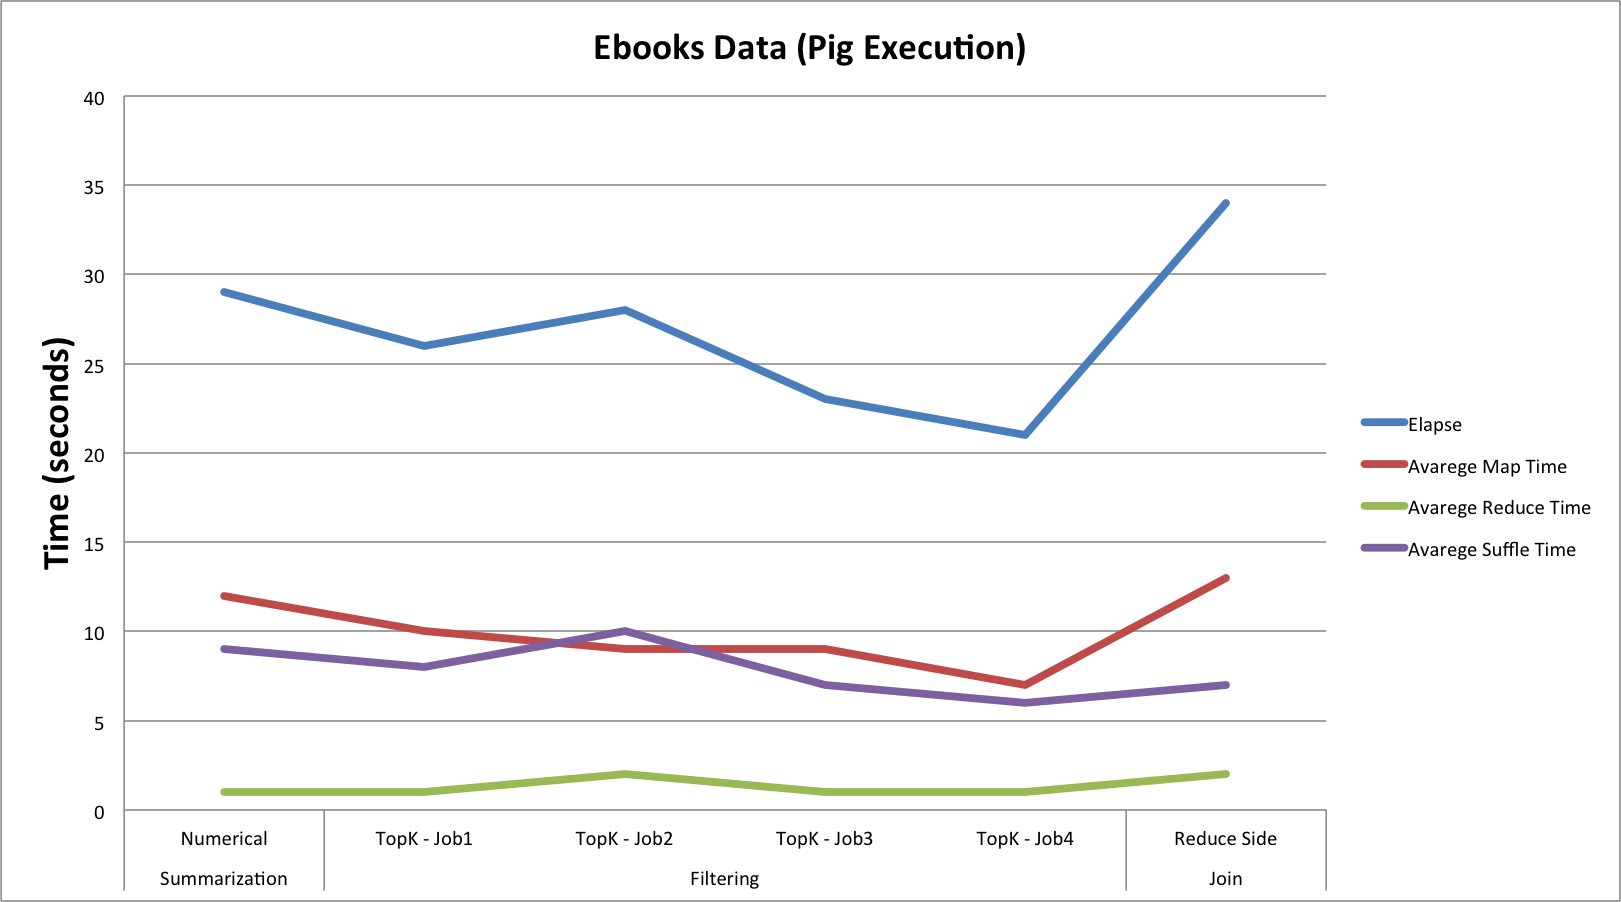
\includegraphics[width=0.471\textwidth]{figs/analysis-charts/pig/ebooks.png}}   
  \subfloat[\textit{Tex} Data]
  {\label{fig:pisp7}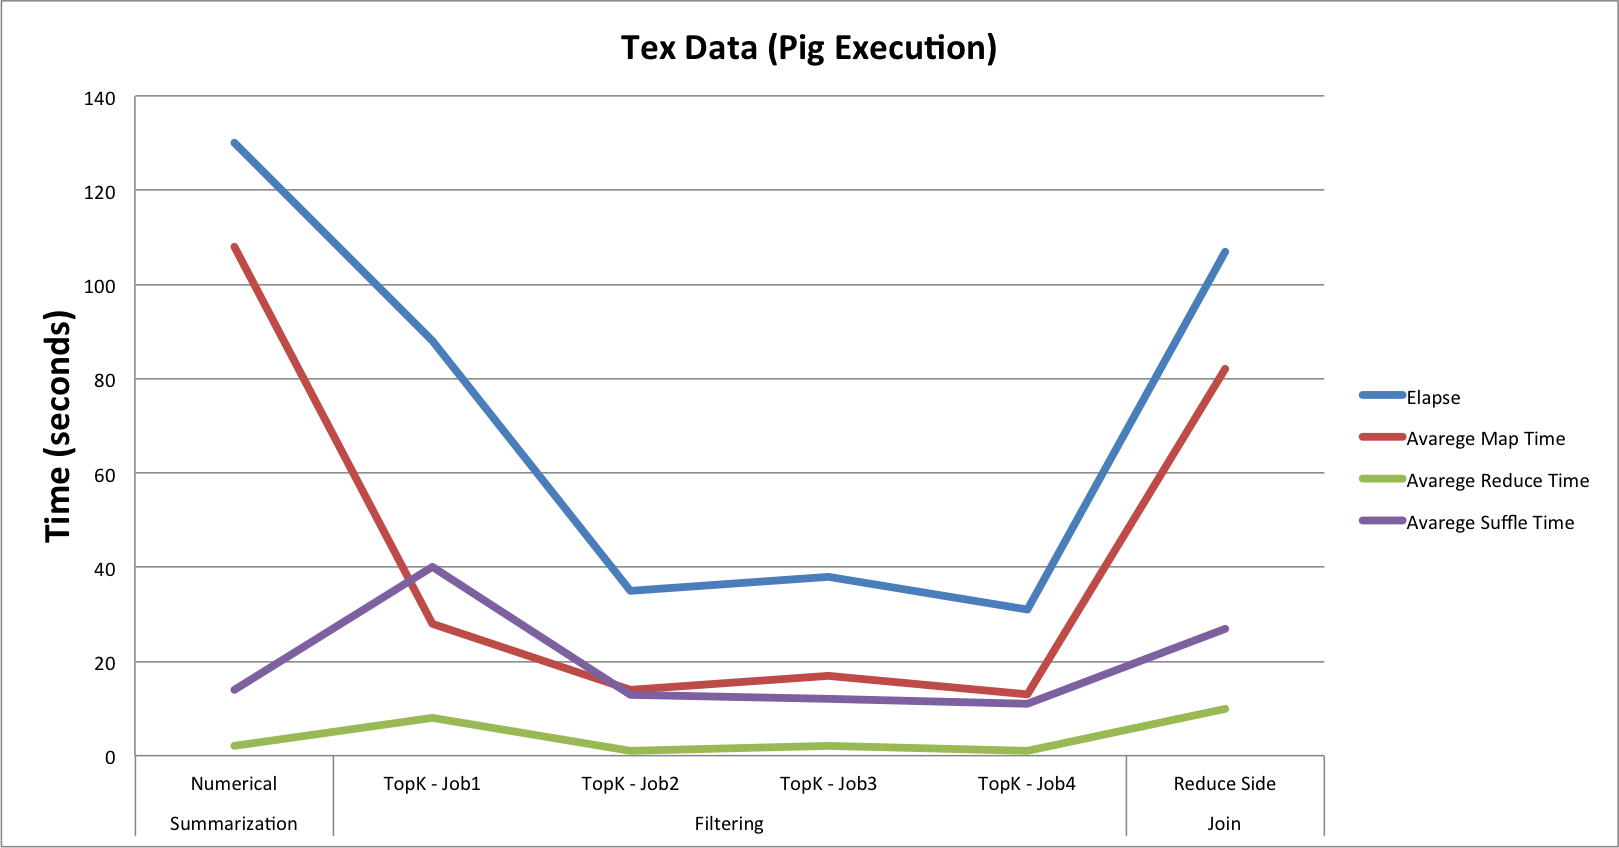
\includegraphics[width=0.5\textwidth]{figs/analysis-charts/pig/tex.png}}
   %add desired spacing between images, e. g. ~, \quad, \qquad etc. (or a blank line to force the subfig onto a new line)
  %~
  \\
  \subfloat[\textit{Serverfault} Data]
  {\label{fig:pisp6}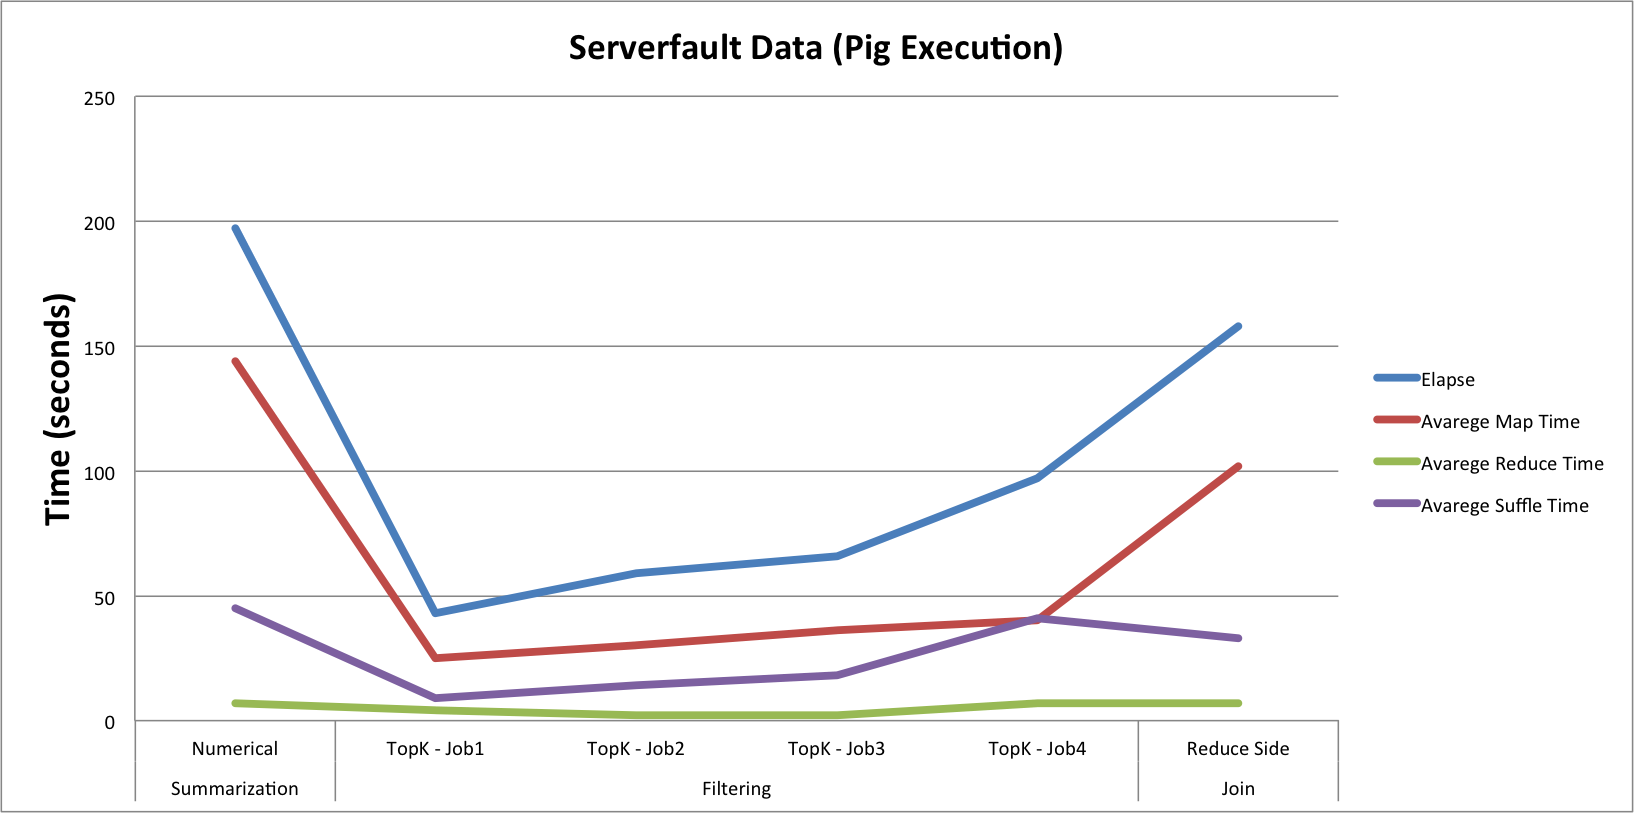
\includegraphics[width=0.5\textwidth]{figs/analysis-charts/pig/serverfault.png}}   
  \subfloat[\textit{Wordpress} Data]
  {\label{fig:pisp7}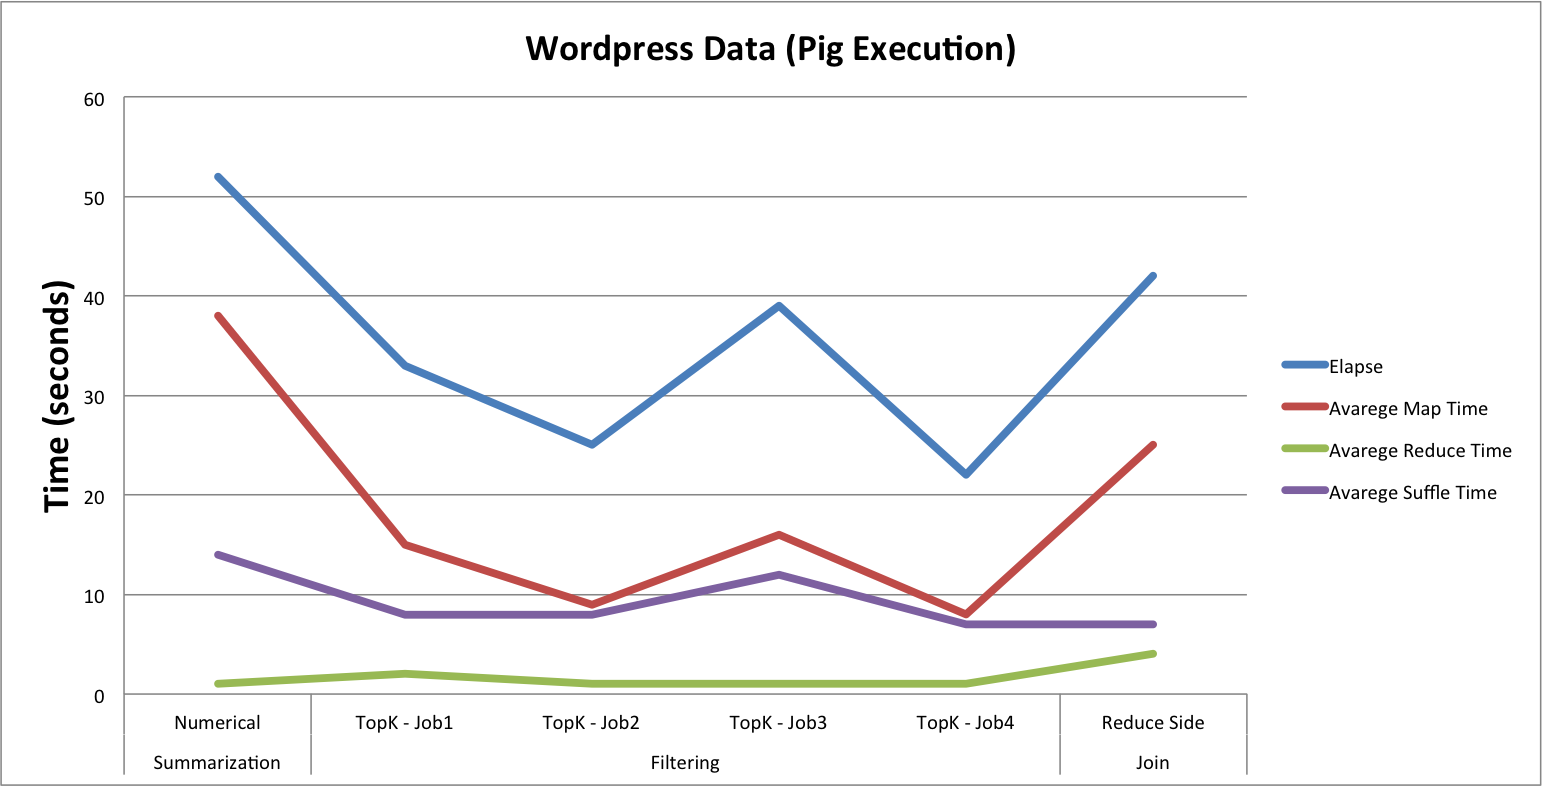
\includegraphics[width=0.49\textwidth]{figs/analysis-charts/pig/wordpress.png}}
   %add desired spacing between images, e. g. ~, \quad, \qquad etc. (or a blank line to force the subfig onto a new line)
  %~
  \\
  \subfloat[\textit{Webapps} Data]
  {\label{fig:pisp8}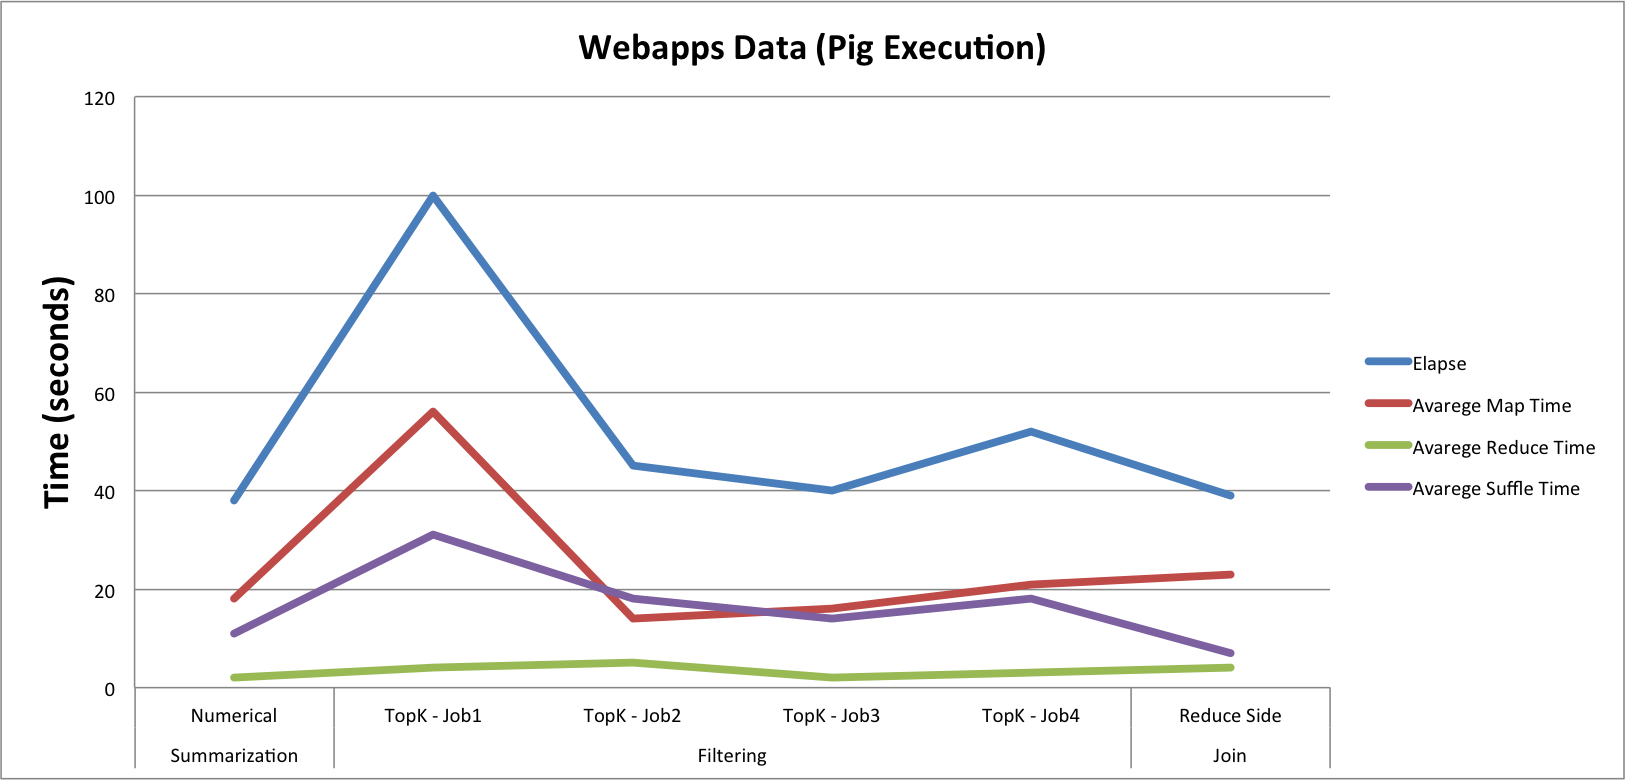
\includegraphics[width=0.5\textwidth]{figs/analysis-charts/pig/webapps.png}}
  ~ %add desired spacing between images, e. g. ~, \quad, \qquad etc. (or a blank line to force the subfig onto a new line)
 
  \caption{MapReduce Design Patterns Performance - Pig Execution.}
  \label{fig:pigexecution}
\end{figure}     
     
\begin{figure}[ht!]
 \centering 
  \subfloat[\textit{Ebooks} Data]
  {\label{fig:pisp6}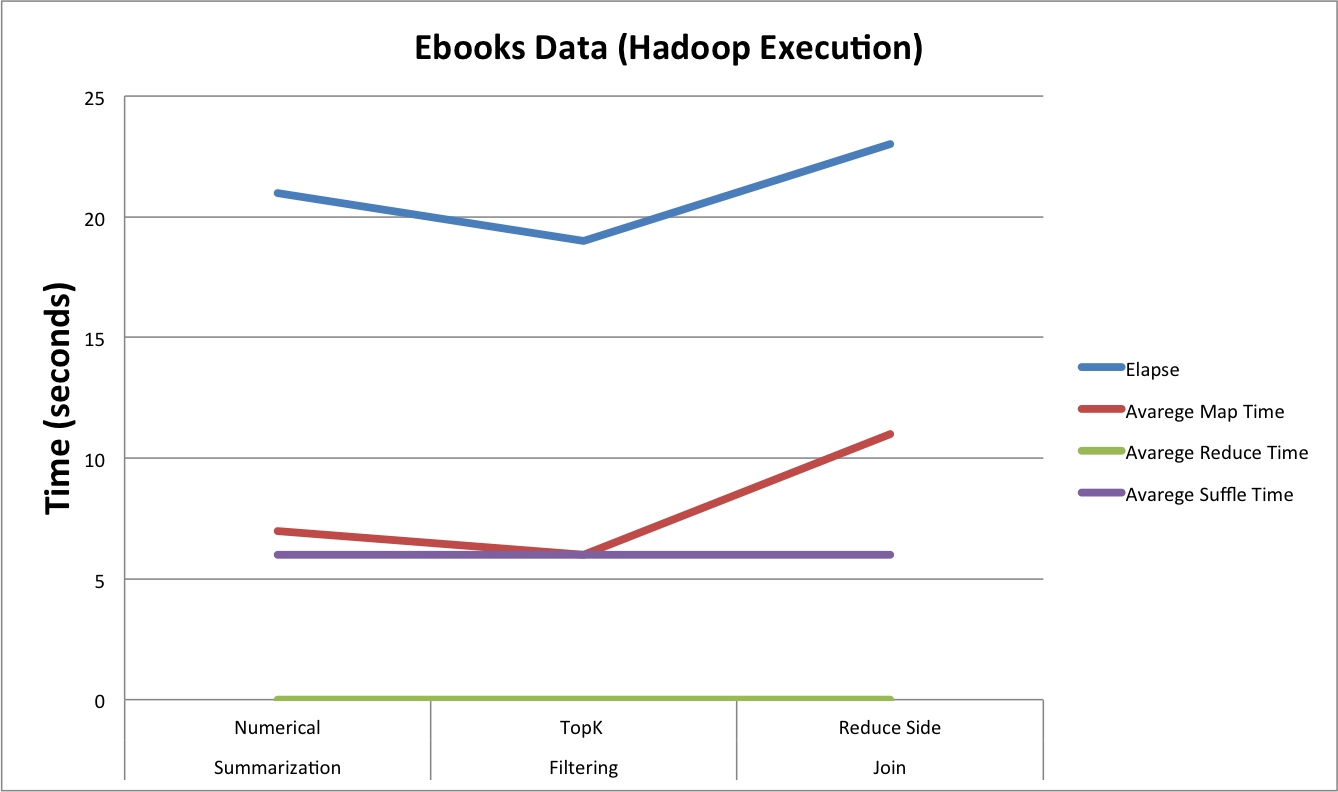
\includegraphics[width=0.456\textwidth]{figs/analysis-charts/hadoop/ebooks.png}}   
  \subfloat[\textit{Tex} Data]
  {\label{fig:pisp7}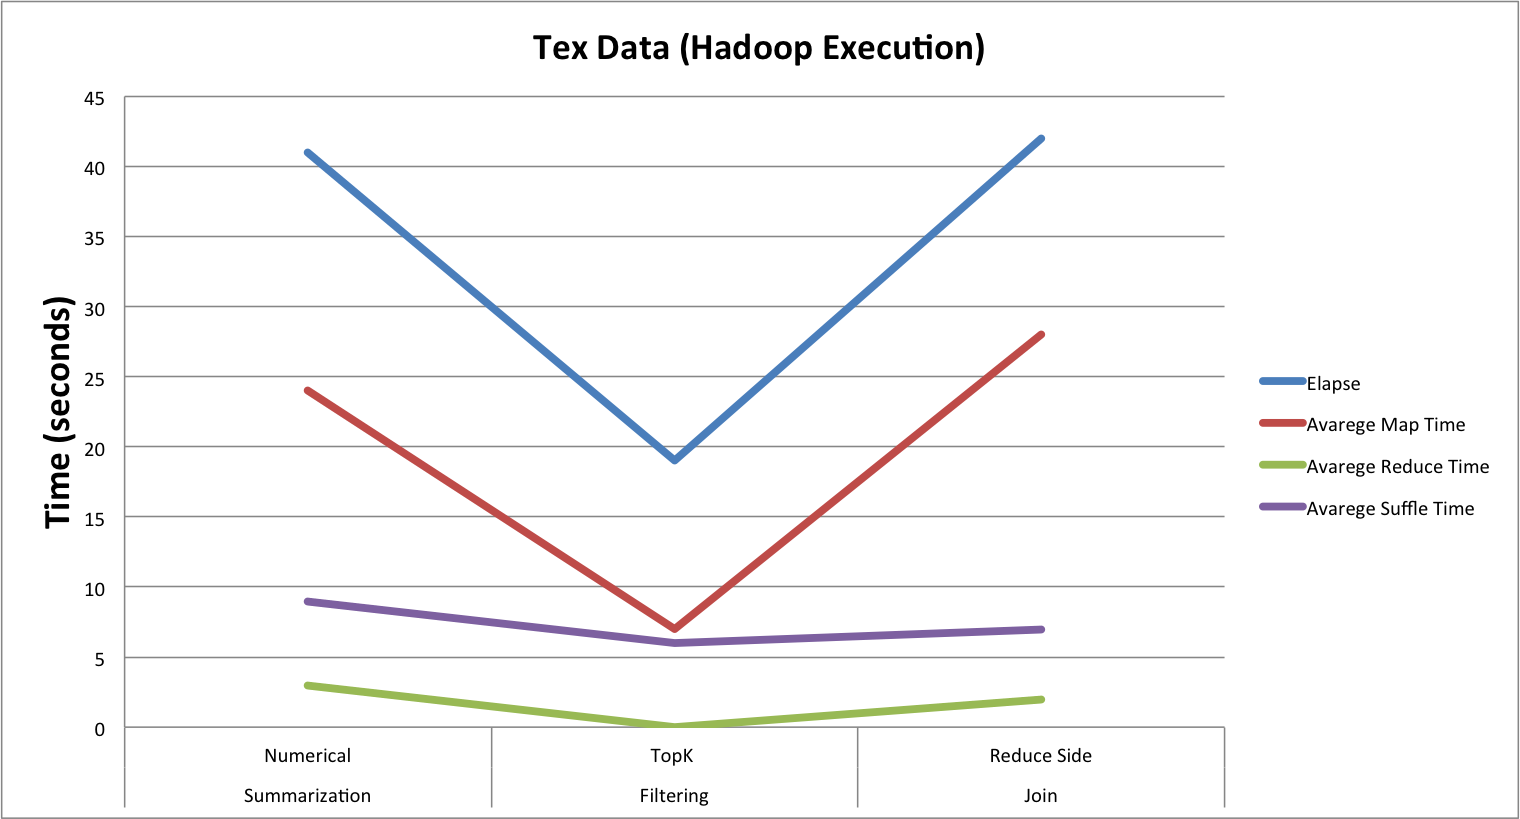
\includegraphics[width=0.5\textwidth]{figs/analysis-charts/hadoop/tex.png}}
   %add desired spacing between images, e. g. ~, \quad, \qquad etc. (or a blank line to force the subfig onto a new line)
  %~
  \\
  \subfloat[\textit{Serverfault} Data]
  {\label{fig:pisp6}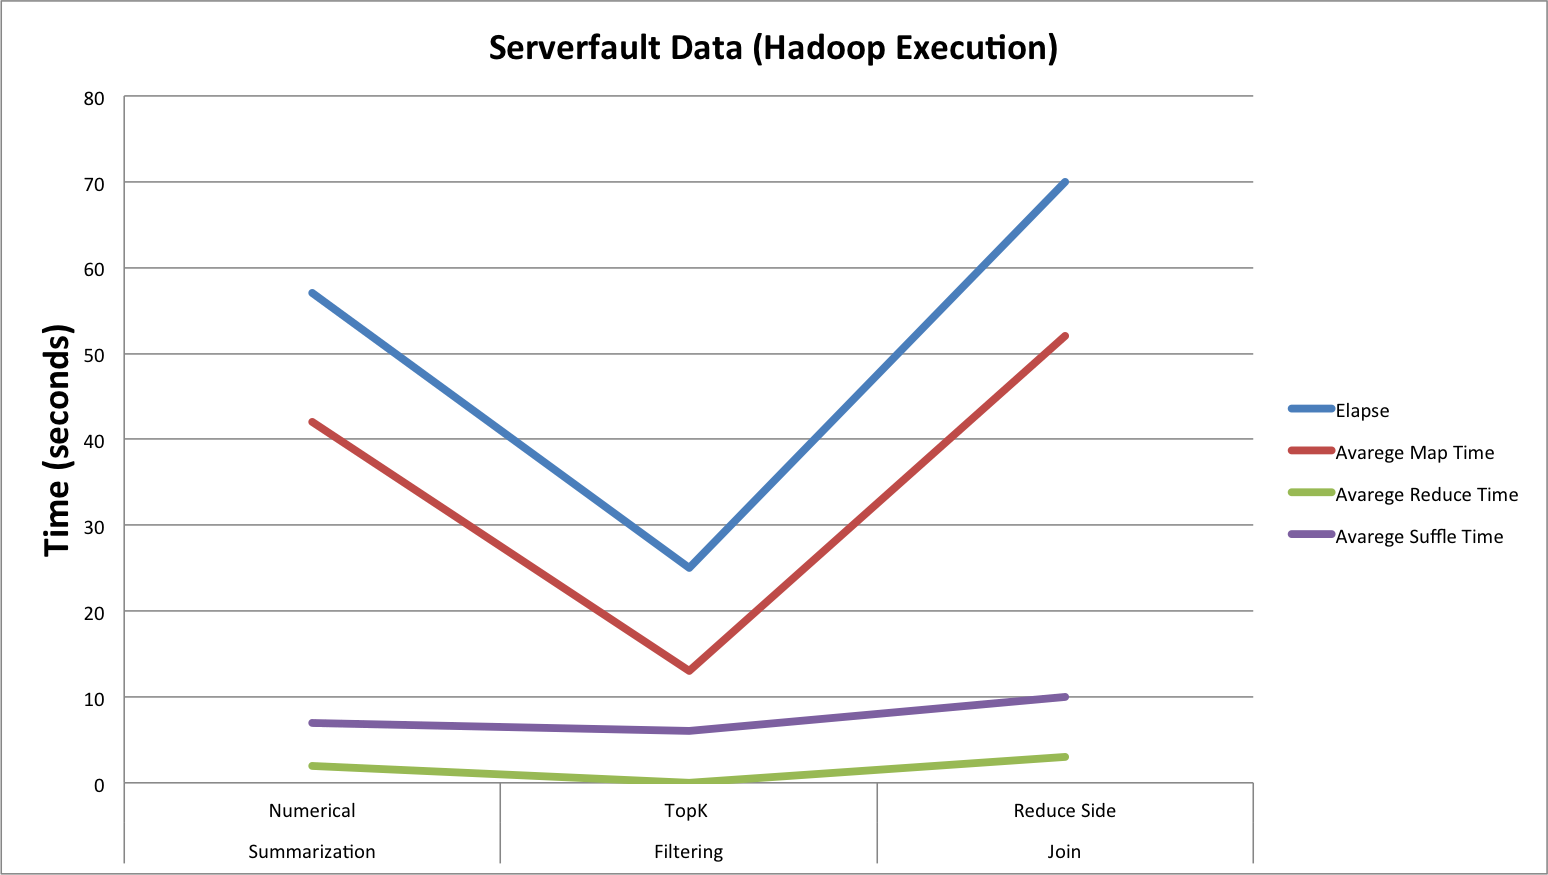
\includegraphics[width=0.485\textwidth]{figs/analysis-charts/hadoop/serverfault.png}}   
  \subfloat[\textit{Wordpress} Data]
  {\label{fig:pisp7}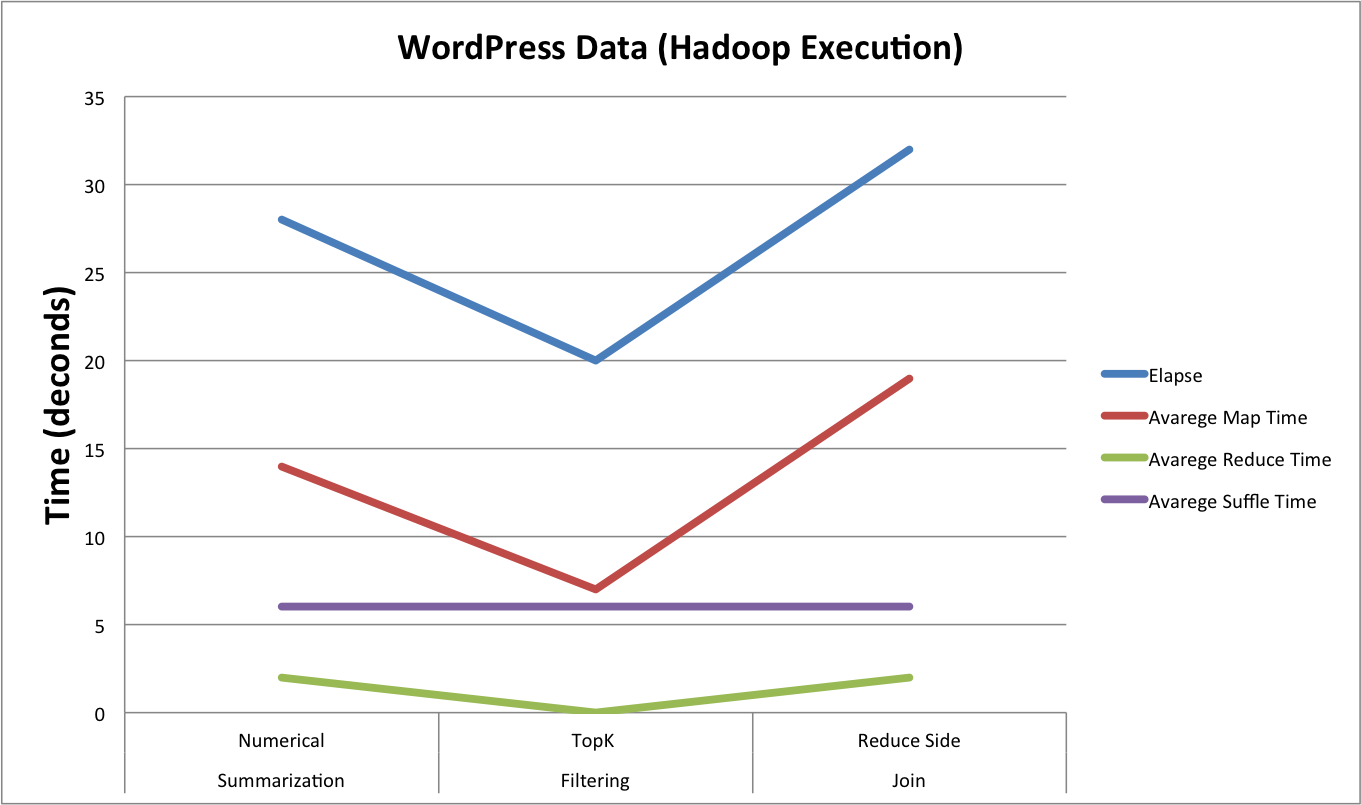
\includegraphics[width=0.466\textwidth]{figs/analysis-charts/hadoop/wordpress.png}}
   %add desired spacing between images, e. g. ~, \quad, \qquad etc. (or a blank line to force the subfig onto a new line)
  %~
  \\
  \subfloat[\textit{Webapps} Data]
  {\label{fig:pisp8}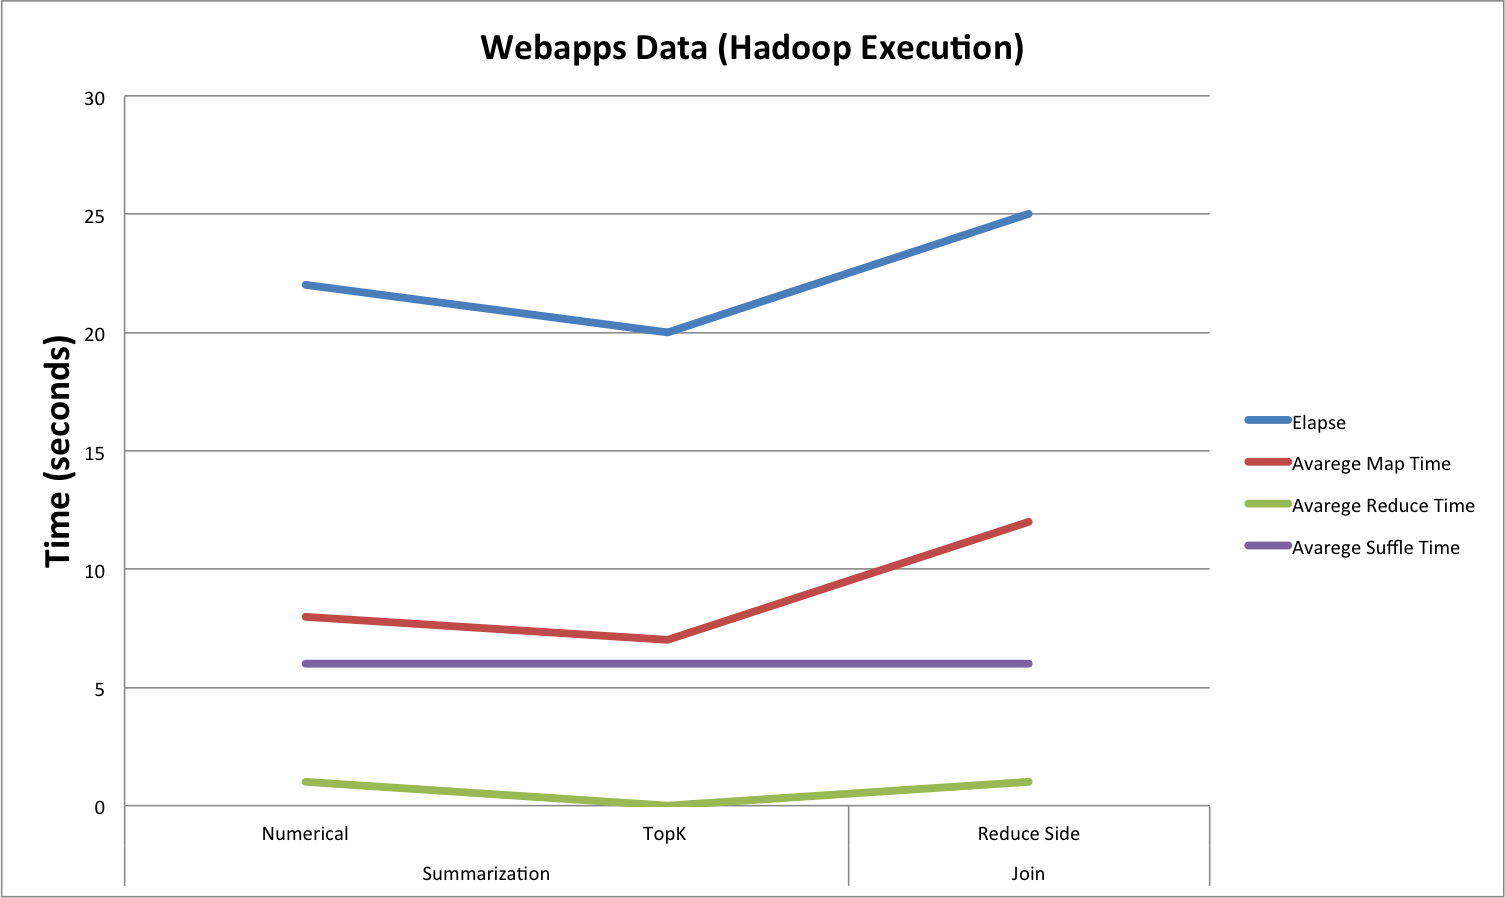
\includegraphics[width=0.5\textwidth]{figs/analysis-charts/hadoop/webapps.png}}
  ~ %add desired spacing between images, e. g. ~, \quad, \qquad etc. (or a blank line to force the subfig onto a new line)
  
  \caption{MapReduce Design Patterns Performance - Hadoop Execution.}
  \label{fig:hadoopexecution}
\end{figure}
   
   
       \begin{figure}[ht!]
 \centering 
 \subfloat[Mappers for Pig Execution]
  {\label{fig:mapperspig}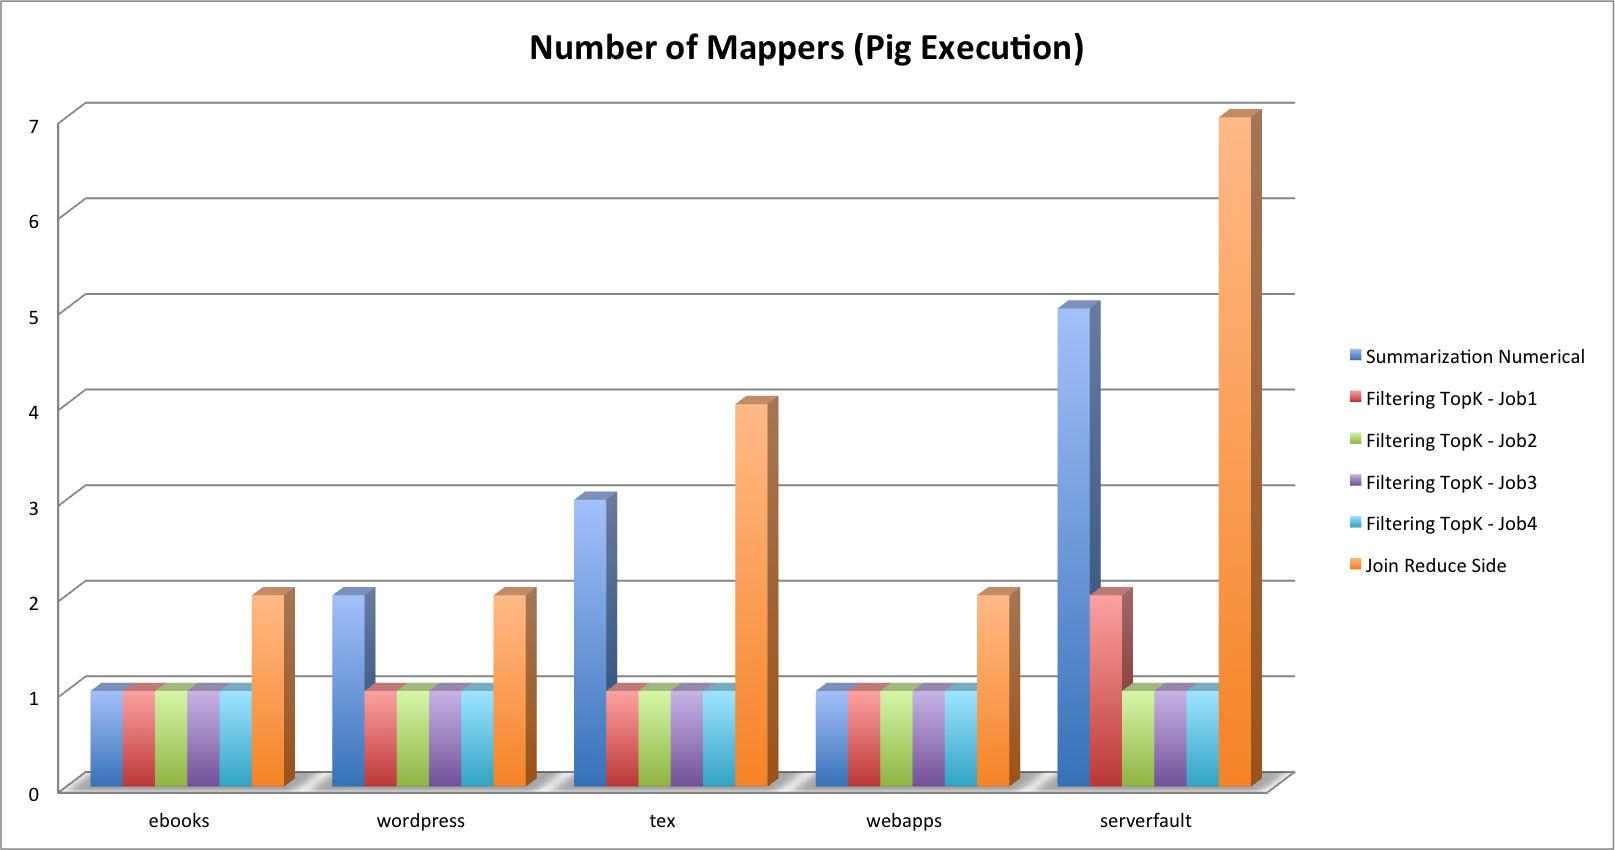
\includegraphics[width=0.6\textwidth]{figs/analysis-charts/pig/mappers.png}}
   %add desired spacing between images, e. g. ~, \quad, \qquad etc. (or a blank line to force the subfig onto a new line)
  %~
  \\
  \subfloat[Mappers for Hadoop Execution]
  {\label{fig:mappershadoop}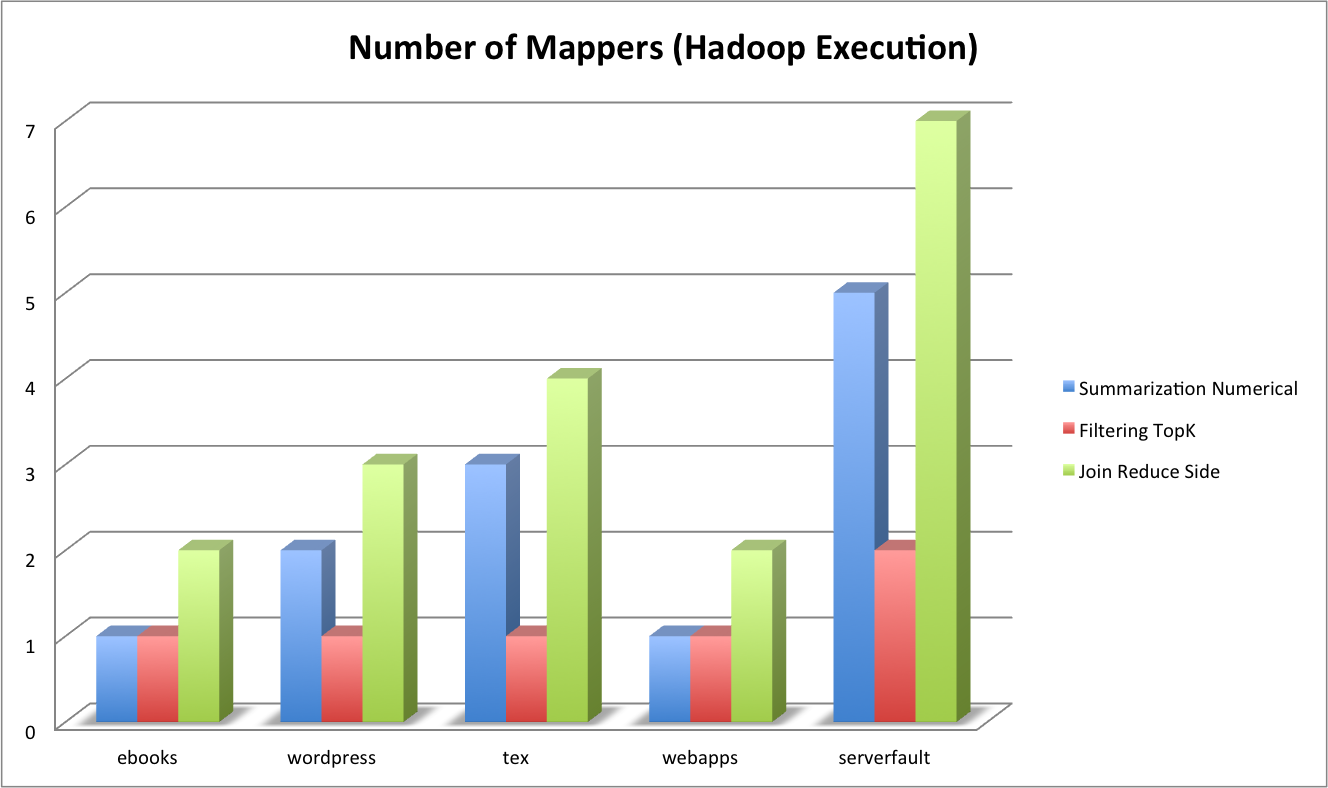
\includegraphics[width=0.6\textwidth]{figs/analysis-charts/hadoop/mappers.png}}
  ~ %add desired spacing between images, e. g. ~, \quad, \qquad etc. (or a blank line to force the subfig onto a new line)
 
  \caption{Number of Mappers - Pig and Hadoop Execution.}
  \label{fig:mappers}
\end{figure}
 
    

\section{Unifying Design Patterns Concepts - Towards a New
Catalogue}\label{sec:catalogue}
\input{catalogue}

\section{Conclusions}\label{sec:conclusions}
\input{conclusions}
 
%% References with bibTeX database:
\bibliographystyle{plain}
\bibliography{bibliography,retrieved-works}


\end{document}

%%
%% End of file `elsarticle-template-1a-num.tex'.
